\chapter{Problem description}\label{ch:problem_desc}
% News & generic usage
While mobile devices have become ubiquitous and powerful for spreading digital information quickly, present-day commercial services and centralized infrastructure pose risks with regard to freedom and privacy.
In this chapter, these risks are discussed in more detail, we explain how fully decentralized distributed solutions can help to increase resilience, and we present the contributions of this thesis.

\section{Privacy and censorship}
%% Censorship
Pervasive monitoring of digital citizens by Internet providers on behalf of governments to enforce censorship laws raises severe privacy concerns \cite{nsa_privacy}.
% Large scale monitoring
The lack of anonymity becomes a problem when the users' privacy is being invaded.
Revealing personal information can be deduced from search queries for example, or associations on social platforms.
When this information can be used for targeted advertising it becomes very valuable, and creates an incentive for the parties that have access to this information to sell it to third parties.
%% Invasion of privacy
Social media companies use targeted advertisement as part of their business model.
Information considered private by users of social media is actually used to broker targeted advertisements.
Subsequently, users can be confronted with their information being misused in various ways beyond their control.
This lack of control over your own privacy can lead to arbitrary interference as defined in UDHR article 12 \cite{UDHR}.
Integration of social media on regular websites makes every page-view and click on these websites traceable to an individual, directly benefiting the business model of targeted advertisements
In fact, the business model of social media appears to be serving targeted advertisements to its users on behalf of third parties.
Even more risk for violation of privacy, comes from integrating social media into regular websites, to de-anonymize and track the whereabouts of users even outside of the realm of social media.
Whenever users lose control over their privacy, it becomes a serious problem.

% Dissent
The incentive to de-anonymize the user, not only causes a lack of privacy, but also a potential lack of freedom of expression, as it hands key information to a censor: who is expressing dissent and who is associated with this person on-line.
Cyber-suppression has become a reality when you no longer can be associated with opinion-makers or foreign journalists on-line.

% Single point of entry
Internet exchange (IX) infrastructures are among the central components in the inter-network architecture that are also vulnerable to monitoring, censorship and Internet kill-switches.
As such, not everyone has unrestricted access to the Internet due to censorship and surveillance.
In fact a significant part of today's Internet users is affected by these attempts to hide or distort reality. %ref
This interference directly affects the universal right to freedom of opinion and expression as stated in article 19 of the Universal Declaration of Human Rights (UDHR) \cite{UDHR}.

During the Arab Spring, Internet kill switches were employed, and within half an hour nearly all networks were unreachable in Egypt in 2011 \cite{renesys2011egypt} and Syria in 2012 \cite{renesys2012syria}.
Other examples of government-imposed censorship with regard to Internet traffic took place in Iran \cite{halderman2013iran}, China \cite{nyt2015appleChina, hrw2006china}, Cuba \cite{watts2014havana} and Turkey \cite{twitter2015turkey}.

The sophistication of censorship techniques is pushed forward by the drive to stay ahead of attempts trying to circumvent it.
Increasingly though, Internet traffic is put under surveillance and obfuscation techniques are targeted by restrictions. \cite{survey_brussee}


\section{Adversary model}\label{sec:adversary_model}
From the Arab Spring scenario we know Internet kill switches are real, so we must assume the existence of a powerful adversary.
The following threats \cite{ietf-shadow-internet} have been identified for similar circumstances:
\begin{itemize}
\item{
	The adversary can observe, block, delay, replay, and modify traffic on the underlying network.
	Thus end-to-end security must not rely on the security of the underlying network.
}
%\item{
%	Wireless communication is regularly monitored.
%	Responding to any wireless requests from a stranger is a direct threat to the user and extremely harmful.
%}
%\item{
%	Possession of encrypted electronic messages or encryption technology in general is extremely harmful to the smartphone owner.
%}
\item{
	The adversary has a limited ability to compromise smartphones or other participating devices.
	If a device is compromised, the adversary can access any information held in the device's volatile memory or persistent storage.
}
\item{
	The adversary can choose the data written to the transport layer by higher protocol layers.
}
\item{
	The adversary cannot break standard cryptographic primitives, such as block ciphers and message-authentication codes.
}
\end{itemize}
%Encryption is not a sufficient requirement of the friend-to-friend scenario, everything MUST be hidden.
%Possession of smartphones apps with encryption is already dangerous for the owner.
We assume the adversary cannot eavesdrop, jam, delay, replay, modify or spoof wireless communication between smartphones.
The adversary cannot compromise smartphones or other participating devices.
%Sybil?

\begin{figure}[H]
	\centering
	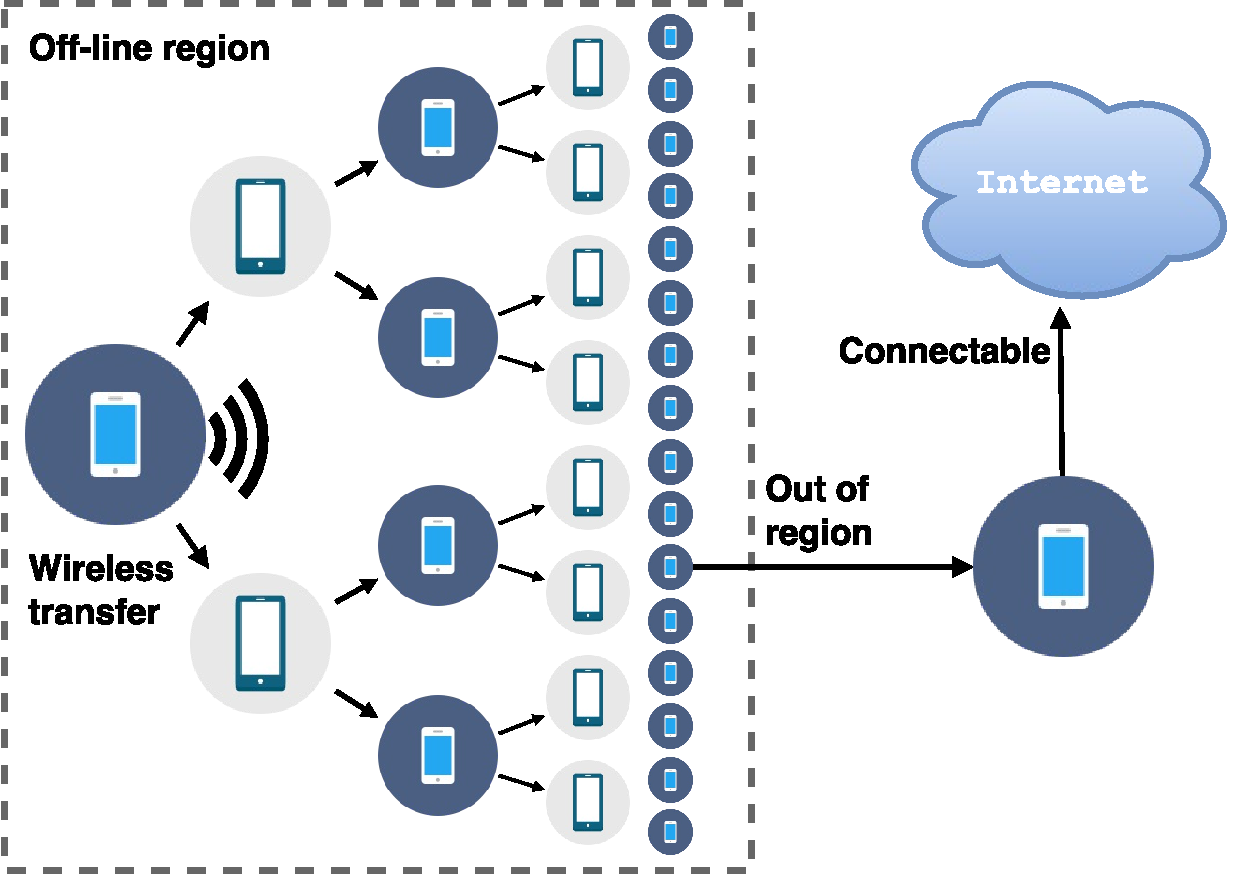
\includegraphics[width=0.7\textwidth]{viral_spreading}
	\caption{Viral spreading from one device to another within an off-line region}
	\label{fig:viral_spreading}
\end{figure}


\section{Distributed solutions}\label{sec:distributed_solutions}
%TODO: van een algemene naar specifieke case:
%- fully distributed oplossingen geven meer resilience tegen kill switches etc
%- mobiele oplossingen geven nog meer resiliency en zijn dus belangrijk om mogelijk te maken
%- zie plaatje: er is nog geen bruikbare oplossing
%- Tribler is een fully distributed systeem ontwikkeld op TUD
%- we gaan nu Tribler op mobiel mogelijk maken. Van "the only way to take Tribler down is to take the Internet down" naar "the only way...take everybody's smartphones away"
With distributed solutions, a scenario like in Figure \ref{fig:viral_spreading} would become possible.
Mobile devices can freely move around off-grid, and eventually one or more devices will move out of the off-line region, also known as "the freedom border".

To ensure that no controlling party can exercise censorship, authority must be distributed over all users. % creating an \emph{autonomous} system.
If all information is located in one or a few places, the parties in charge of that location will still have control over it, so information must be distributed over all users as well, creating a \emph{communication} system.
Finally, all users must be able to share, order and appreciate information of other users, in other words the essence of social media: social interaction.
With everyone being able to interact in the same way we need to  distribute functionality over all users, creating a \emph{cooperation} system.
% Solution
Fully distributed systems capture the characteristics just mentioned.

Therefore, to render the effect mute of the Internet kill switches in existence, distributed solutions will be essential.
Without any central component in the system, it becomes difficult to censor effectively without everyone participating.

The following network properties are defined \cite{hasan2013dissent} to provide a technical solution that enables free expression in the face of an adversary as defined in Section \ref{sec:adversary_model}:
\begin{itemize}
	\item \emph{Resilient against communications blackouts.}
	Should be challenging for any entity to disable.
	\item \emph{Resistant to monitoring and tracking of users.}
	Both who is using the network and any sensitive messages they send should be secret.
	\item \emph{Able to be built from innocuous components.}
	Should only require readily available hardware, and the possession and use of required hardware should not be illegal or suspicious.
	\item \emph{Able to run at meaningful scales.}
	Should be more effective at disseminating information than people with megaphones; more broadly, given a level of service, should be able to run at non-trivial scales.
\end{itemize}

Tribler, which has been developed as a non-profit research project at Delft University of Technology, has been proposed as a solution to realize an information sharing platform that protects the privacy of its users and is resilient to attacks \cite{tor_bittorrent}.
Thanks to the server-less design we can say: \emph{The only way to take Tribler down is to take the entire Internet down.}

Including mobile devices in this context is crucial.
The ubiquity of these devices will be beneficial for viral spreading of information, as shown in Figure \ref{fig:viral_spreading}.
At the same time, this ubiquity will also allow the creation of a fully decentralized social network.
When bringing Tribler's functionality to mobile devices, with regard to resilience against censorship, an important next step will be taken, so we can say: \emph{Even if you can take down the Internet, the only way to take Tribler down is to take everybody's smartphones away.}
% Eindig aantal servers points of failures

Peer-to-peer communication technology is essential for a server-less distributed system.
Mobile devices usually are already well equipped to exchange information without reliance on external infrastructure, for example through Bluetooth or ad hoc Wi-Fi or near-field communication (NFC).
Therefore, they will be even more suitable as a solution for communicating peer-to-peer than PC.

\begin{figure}
	\centering
	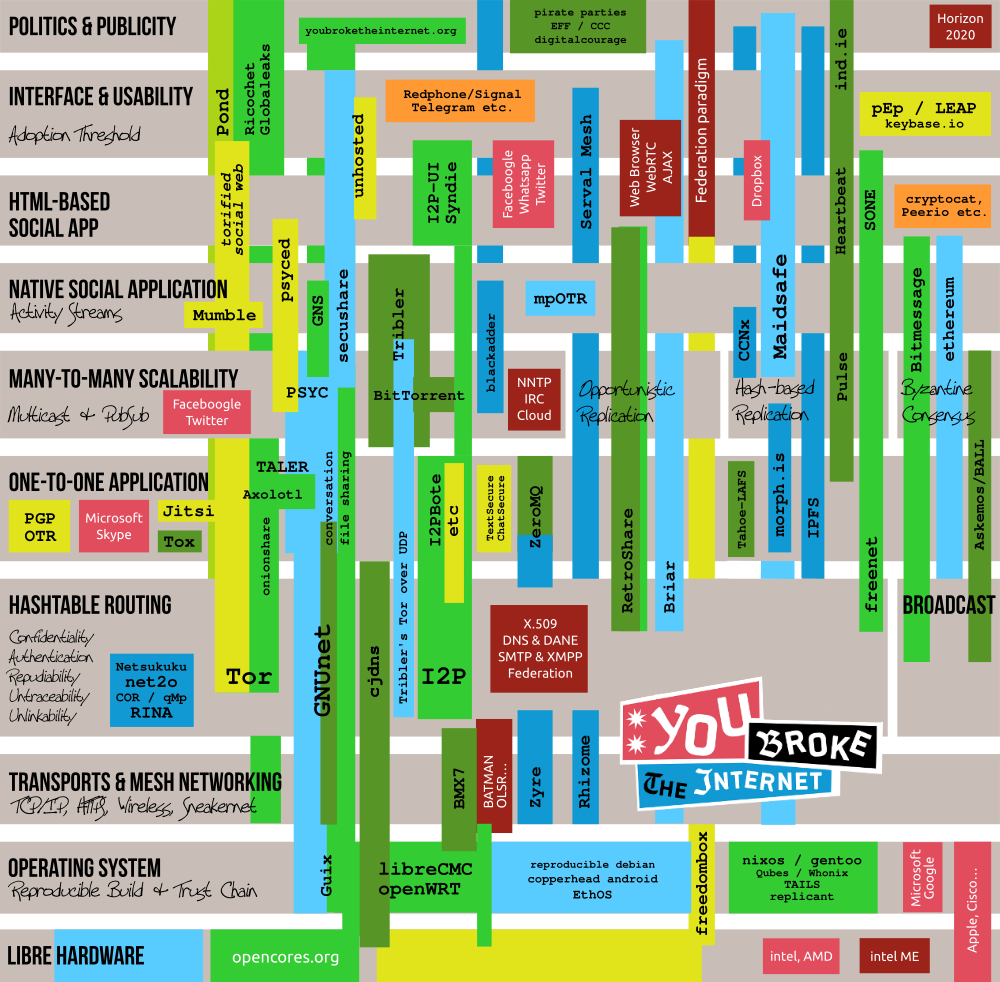
\includegraphics[width=\textwidth]{youbroketheinternet}
	\caption{Various partial solutions to mend the broken Internet according to www.youbroketheinternet.org}
	\label{fig:youbroketheinternet}
\end{figure}

% Fragmented
The urgency for enabling attack-resilient media exchange on mobile devices becomes even stronger, considering that no de-facto solutions are available for this yet \cite{redecentralize2015alternativeinternet, survey_brussee}.
As shown in Figure \ref{fig:youbroketheinternet}, various solutions have been proposed, but none of them provide a full solution.


\section{Contributions}
% requirements analysis
% maintainable design & implementation
% performance analysis
Leveraging the properties of mobile devices like smartphones, together with the features of Tribler, we see a perfect match to enable attack-resilient media via phone-to-phone networking.
However, previous attempts to bring Tribler to mobile did not deliver all functionality yet \cite{tribler2014play,tribler2014at3,tribler-anon-hd}.
Maintainability issues with earlier designs and large amounts of technical debt were the major causes \cite{thesis_martijn}.
We changed the architecture of Tribler for our approach.

The work in this thesis now provides the first prototype implementation that has all Tribler functionality fully enabled on mobile devices.
The prototype has been designed for portability and maintainability.
Our experiments will verify the feasibility of running Tribler on mobile devices.
Generally, by enabling future research with Tribler fully geared towards mobile devices, the prototype makes an important contribution to the field.

%The main contribution of this thesis is making Tribler available on mobile devices and the utilization of their unique properties in the context of censorship and communication during crises.
%This work also enables a new direction for future research with Tribler: mobile devices.
%The scientific contributions of this work are the experiments to verify the feasibility of Tribler on mobile devices and the ability to perform research with Tribler fully geared towards mobile devices.

